\documentclass[../main.tex]{subfiles}

\begin{document}
\section{Results}\label{sec:results}

\subsection{The bias-variance tradeoff}
With a dataset of values produced from Franke's function, we've fitted a model based on the training set and predicted new data based on the testing set. This was done with a design matrix of increasing degrees, from $1$ to $9$. The following figure \ref{fig:result_complexity} is a plot relating the mean squared error of the model to the complexity (or degree).

\begin{figure}[h]
    \centering
    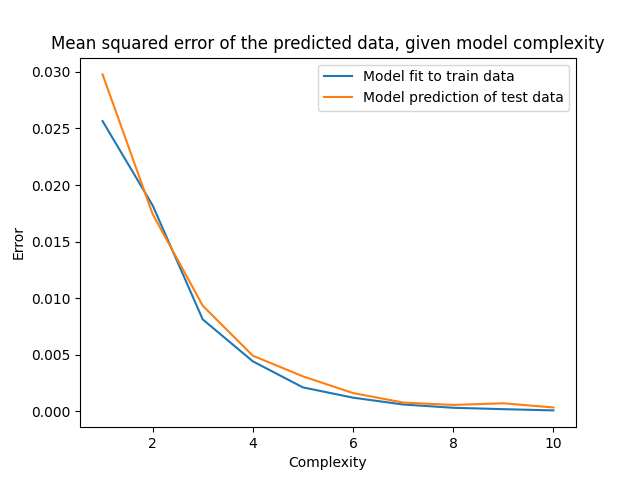
\includegraphics[width=\textwidth]{../assets/complexity.png}
    \caption{The error of a model based on the train and test set respectively, in relation to the degree of the model.}
    \label{fig:result_complexity}
\end{figure}

\begin{figure}[htb] 
   \centering
   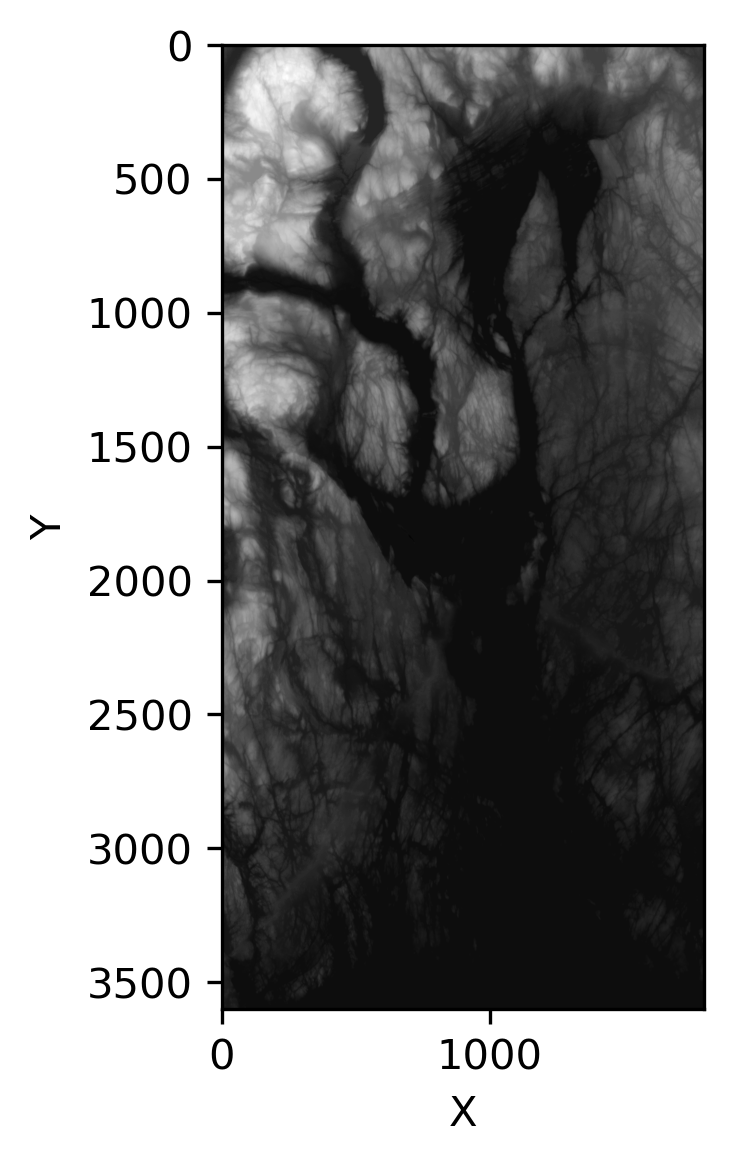
\includegraphics[width=0.4\textwidth]{../assets/terrain_n59_e010.png} 
   \caption{Terrain data over Norway 59\degree north, 10\degree east.}
   \label{fig:terrain_Norway}
\end{figure} 

\end{document}
